\documentclass[lettersize, journal]{IEEEtran}
\usepackage[utf8]{inputenc} 
\usepackage[T1]{fontenc}   
\usepackage{mathptmx}       
\usepackage{graphicx}      
\usepackage{float}          
\usepackage{algorithmic}
\usepackage{algorithm}
\usepackage{caption}        
\usepackage{subcaption}     
\usepackage{biblatex}       
\usepackage{amsmath, amsfonts, amssymb}  
\usepackage{hyperref}       

\addbibresource{reference.bib} 



\begin{document}

% Paper title
\title{Data-Driven Forecasting of Mechanical Ventilator Demands: A Deep learning of COVID-19 Data in England}
\author{Michael Ajao-olarinoye}

\maketitle
\thispagestyle{empty}


\begin{abstract}
    This document describes the most common article elements and how to use the IEEEtran class with \LaTeX \ to produce files that are suitable for submission to the IEEE.  IEEEtran can produce conference, journal, and technical note (correspondence) papers with a suitable choice of class options.
\end{abstract}

\begin{IEEEkeywords}
    Article submission, IEEE, IEEEtran, journal, \LaTeX, paper, template, typesetting.
\end{IEEEkeywords}

\section{Introduction}
\IEEEPARstart{T}{his} introduce your topic and the purpose of your paper.



\section{Literature Review}
\label{sec:lit_review}
This section should contain a review of the literature relevant to your topic. You should cite the relevant literature in this section. For example, \cite{ajao2020}.

\section[short]{Data analysis}
\begin{figure}[h]
    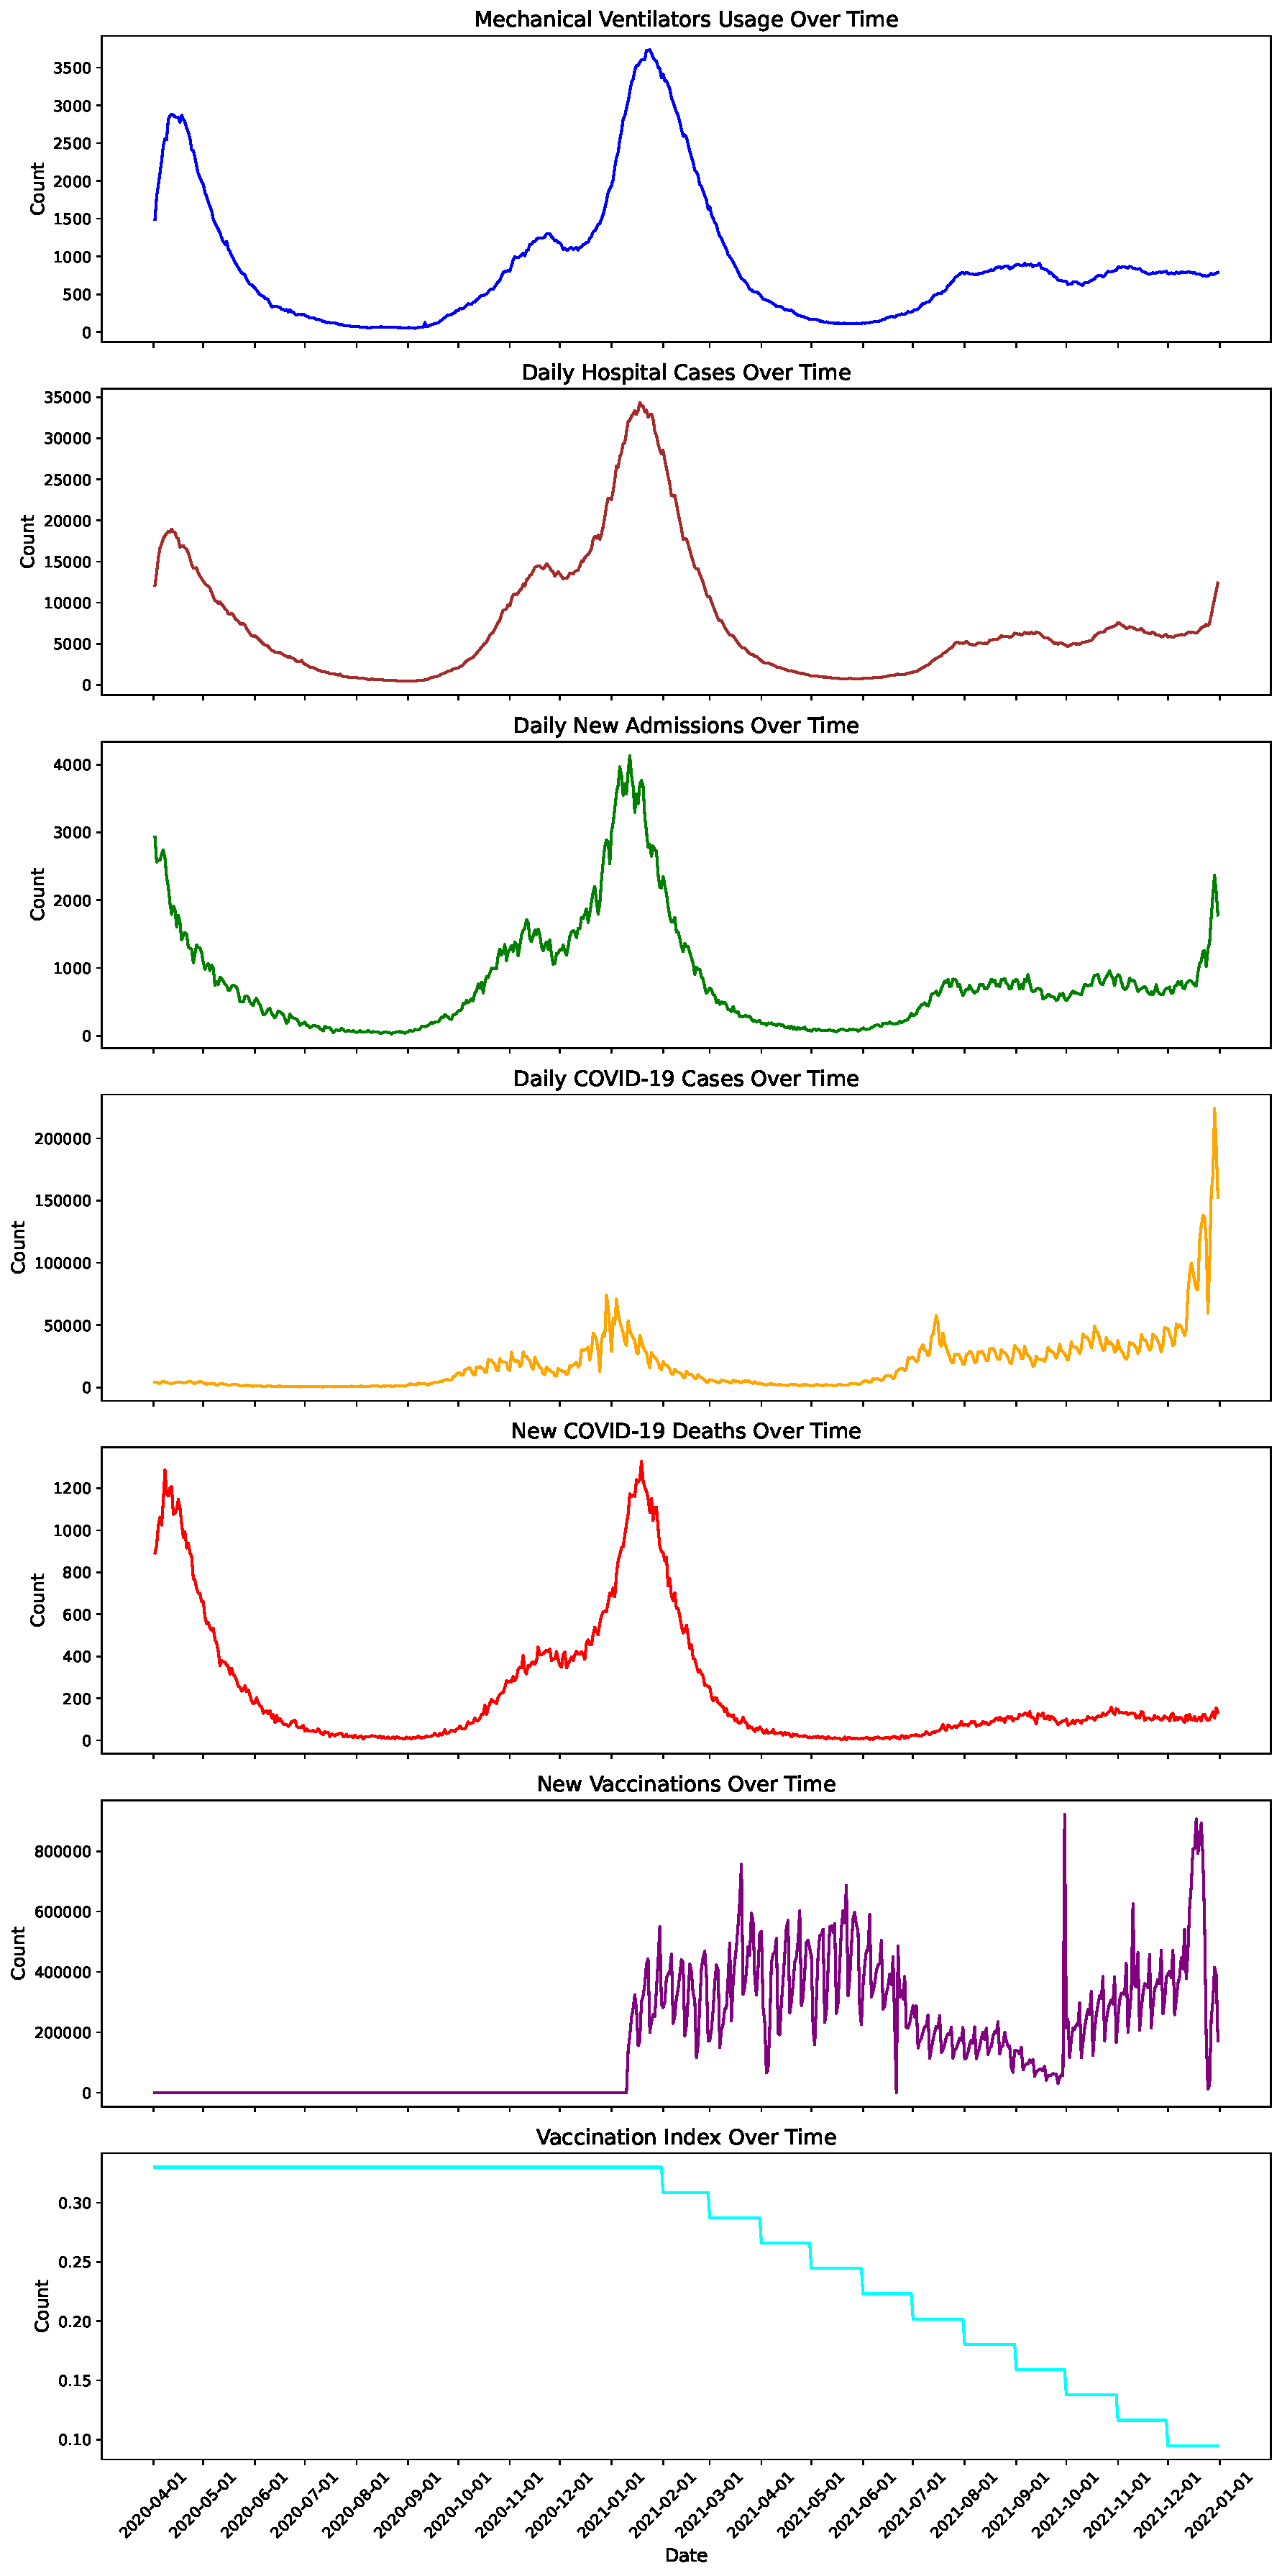
\includegraphics[width=0.4\textwidth]{"../Research paper/images/trend_analysis_improved.pdf"}
\end{figure}

\section{Methodology}
\label{sec:methodology}
This section should contain a description of the methodology used in your work. You should also include the mathematical formulation of your model in this section. For example, the mathematical formulation of the model in \cite{ajao2020} is given by equation \ref{eq:1}.
\begin{equation}
    \label{eq:1}
    \begin{split}
        \min_{\mathbf{w}} \quad & \frac{1}{2} \mathbf{w}^T \mathbf{w} + C \sum_{i=1}^{n} \xi_i \\
        \text{s.t.} \quad & y_i(\mathbf{w}^T \mathbf{x}_i + b) \geq 1 - \xi_i, \quad i = 1, \dots, n \\
        & \xi_i \geq 0, \quad i = 1, \dots, n
    \end{split}
\end{equation}

\section[short]{Deep Learning Model Development}
\label{sec:dl_model}
This section should contain a description of the deep learning model developed in your work. You should also include the mathematical formulation of your model in this section. For example, the mathematical formulation of the model in \cite{ajao2020} is given by equation \ref{eq:2}.

\begin{equation}
    \label{eq:2}
    \begin{split}
        \min_{\mathbf{w}} \quad & \frac{1}{2} \mathbf{w}^T \mathbf{w} + C \sum_{i=1}^{n} \xi_i \\
        \text{s.t.} \quad & y_i(\mathbf{w}^T \mathbf{x}_i + b) \geq 1 - \xi_i, \quad i = 1, \dots, n \\
        & \xi_i \geq 0, \quad i = 1, \dots, n
    \end{split}
\end{equation}

\section{Results and Discussion}
\label{sec:results}
This section should contain the results of your work. You should also discuss the results in this section. For example, the results of the model in \cite{ajao2020} are shown in figure \ref{fig:1}.
% \begin{figure}[H]
%     \centering
%     \includegraphics[width=0.5\textwidth]{figures/fig1.png}
%     \caption{Results of the model in \cite{ajao2020}}
%     \label{fig:1}
% \end{figure}

\section{Conclusion}
\label{sec:conclusion}



\printbibliography


\end{document}
